\documentclass[aspectratio=169]{beamer}

% Theme
\usetheme{default}
\usecolortheme{beaver}

% Packages
\usepackage{amsmath,amssymb,amsthm}
\usepackage{mathtools}
\usepackage{bm}
\usepackage{tikz}
\usetikzlibrary{arrows.meta,positioning,calc,patterns,decorations.markings}

% Custom commands
\newcommand{\R}{\mathbb{R}}
\newcommand{\Z}{\mathbb{Z}}
\newcommand{\Pp}{\mathcal{P}}
\newcommand{\Mm}{\mathcal{M}}
\newcommand{\Ld}{\mathcal{L}^d}
\newcommand{\Hd}{\mathcal{H}^{d-1}}
\newcommand{\Cb}{C_b}
\newcommand{\Czero}{C_0}
\newcommand{\Td}{\mathbb{T}^d}

% Title
\title{Strictly Convex and Quadratic Costs}
\subtitle{Chapter 1.3: Existence of Optimal Transport Maps}
\author{}
\date{}

\begin{document}

%==============================================================================
\begin{frame}
\titlepage
\end{frame}

%==============================================================================
\begin{frame}[shrink=10]{Outline}
\tableofcontents[hideallsubsections]
\end{frame}

%==============================================================================
\section{Introduction and Setup}
%==============================================================================

\begin{frame}{Setting: Strictly Convex Costs}
\textbf{Setting:} $X = Y = \Omega \subset \R^d$ compact, cost of the form:
\[
\boxed{c(x,y) = h(x-y)}
\]
where $h: \R^d \to \R$ is \textbf{strictly convex}.

\vspace{0.3cm}
\textbf{Main goal:} Show existence and uniqueness of an \textbf{optimal transport map} $T$.

\vspace{0.3cm}
\begin{center}
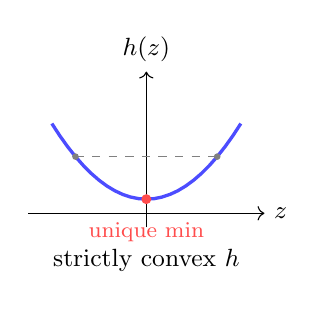
\begin{tikzpicture}[scale=0.6]
    % Strictly convex h
    \draw[->] (-2.5,0) -- (2.5,0) node[right] {\small $z$};
    \draw[->] (0,-0.3) -- (0,3) node[above] {\small $h(z)$};

    % Convex function
    \draw[blue!70, very thick, domain=-2:2] plot (\x, {0.4*\x*\x + 0.3});

    % Unique minimum
    \fill[red!70] (0, 0.3) circle (3pt);
    \node[below, red!70, font=\footnotesize] at (0, 0) {unique min};

    % Strict convexity illustration
    \draw[gray, dashed] (-1.5, 1.2) -- (1.5, 1.2);
    \fill[gray] (-1.5, 1.2) circle (2pt);
    \fill[gray] (1.5, 1.2) circle (2pt);

    \node at (0, -1) {\small strictly convex $h$};
\end{tikzpicture}
\end{center}

\vspace{0.2cm}
\textbf{Key tool:} Duality result $\max(\text{DP}) = \min(\text{KP})$ (Theorem 1.39).
\end{frame}

%==============================================================================
\begin{frame}{Optimality Conditions from Duality}
From an optimal transport plan $\gamma$ and Kantorovich potential $\phi$:
\[
\phi(x) + \phi^c(y) \leq c(x,y) \quad \text{on } \Omega \times \Omega
\]
\[
\phi(x) + \phi^c(y) = c(x,y) \quad \text{on } \text{spt}(\gamma)
\]

\vspace{0.4cm}
\textbf{Interpretation:}
\begin{itemize}
    \item The constraint $\phi \oplus \phi^c \leq c$ is always satisfied
    \item On the support of optimal $\gamma$, the constraint is \textbf{tight} (equality holds)
    \item This characterizes where mass is actually transported
\end{itemize}
\end{frame}

%==============================================================================
\begin{frame}{Why Equality on $\text{spt}(\gamma)$?}
\textbf{From duality:}
\[
\int_{\Omega \times \Omega} c \, d\gamma = \int_\Omega \phi \, d\mu + \int_\Omega \phi^c \, d\nu = \int_{\Omega \times \Omega} (\phi(x) + \phi^c(y)) \, d\gamma
\]

$\Rightarrow$ Equality $\gamma$-a.e., and since $\phi, \phi^c$ continuous, equality on $\text{spt}(\gamma)$.

\vspace{0.3cm}
\begin{center}
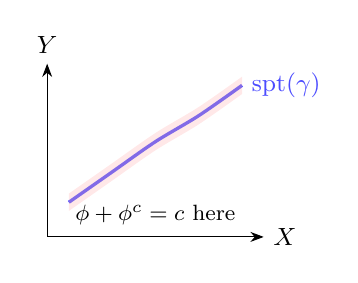
\begin{tikzpicture}[scale=0.55]
    \draw[-{Stealth}] (0,0) -- (5,0) node[right] {\small $X$};
    \draw[-{Stealth}] (0,0) -- (0,4) node[above] {\small $Y$};

    % Support of gamma
    \draw[blue!70, very thick] plot[smooth] coordinates {(0.5,0.8) (1.5,1.5) (2.5,2.2) (3.5,2.8) (4.5,3.5)};
    \node[blue!70, right, font=\small] at (4.5, 3.5) {$\text{spt}(\gamma)$};

    % Equality region
    \fill[red!30, opacity=0.3] plot[smooth] coordinates {(0.5,0.6) (1.5,1.3) (2.5,2) (3.5,2.6) (4.5,3.3)}
        -- plot[smooth] coordinates {(4.5,3.7) (3.5,3) (2.5,2.4) (1.5,1.7) (0.5,1)} -- cycle;

    \node[font=\footnotesize] at (2.5, 0.5) {$\phi + \phi^c = c$ here};
\end{tikzpicture}
\end{center}

\textbf{Key insight:} The support of $\gamma$ lies in the \textbf{contact set} $\{\phi \oplus \phi^c = c\}$.
\end{frame}

%==============================================================================
\section{Support and Gradient Relations}
%==============================================================================

\begin{frame}{Definition 1.14: Support of a Measure}
\begin{block}{Definition (Support)}
On a separable metric space $X$, the \textbf{support} of a measure $\gamma$ is:
\[
\boxed{\text{spt}(\gamma) := \bigcap \{A : A \text{ is closed and } \gamma(X \setminus A) = 0\}}
\]
\end{block}

\vspace{0.4cm}
\textbf{Equivalent characterization:}
\[
\text{spt}(\gamma) = \{x \in X : \gamma(B(x,r)) > 0 \text{ for all } r > 0\}
\]

\vspace{0.3cm}
\textbf{Intuition:} A point $x$ is in the support if every neighborhood of $x$ has positive measure.
\end{frame}

%==============================================================================
\begin{frame}{Support of a Measure: Visualization}
\begin{columns}
\begin{column}{0.55\textwidth}
\textbf{Key property:}

$\gamma$ is concentrated on $\text{spt}(\gamma)$:
\[
\gamma(X \setminus \text{spt}(\gamma)) = 0
\]

\vspace{0.3cm}
\textbf{Examples:}
\begin{itemize}
    \item $\delta_a$: $\text{spt}(\delta_a) = \{a\}$
    \item Uniform on $[0,1]$: $\text{spt} = [0,1]$
    \item Gaussian: $\text{spt} = \R^d$
\end{itemize}
\end{column}
\begin{column}{0.45\textwidth}
\begin{center}
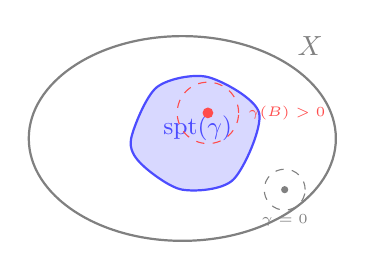
\begin{tikzpicture}[scale=0.65]
    % Space X
    \draw[gray, thick] (0,0) ellipse (3 and 2);
    \node[gray] at (2.5, 1.8) {$X$};

    % Support (where measure lives)
    \fill[blue!30, opacity=0.5] plot[smooth cycle] coordinates {(-1,0) (-0.5,1) (0.5,1.2) (1.5,0.5) (1,-0.8) (0,-1) (-0.8,-0.5)};
    \draw[blue!70, thick] plot[smooth cycle] coordinates {(-1,0) (-0.5,1) (0.5,1.2) (1.5,0.5) (1,-0.8) (0,-1) (-0.8,-0.5)};
    \node[blue!70, font=\small] at (0.3, 0.2) {$\text{spt}(\gamma)$};

    % Point in support
    \fill[red!70] (0.5, 0.5) circle (3pt);
    \draw[red!70, dashed] (0.5, 0.5) circle (0.6);
    \node[red!70, font=\tiny, right] at (1.1, 0.5) {$\gamma(B) > 0$};

    % Point outside support
    \fill[gray] (2, -1) circle (2pt);
    \draw[gray, dashed] (2, -1) circle (0.4);
    \node[gray, font=\tiny] at (2, -1.6) {$\gamma = 0$};
\end{tikzpicture}
\end{center}
\end{column}
\end{columns}
\end{frame}

%==============================================================================
\begin{frame}{Proposition 1.15: Gradient Relation}
\begin{block}{Proposition 1.15}
If $c$ is $C^1$, $\phi$ is a Kantorovich potential, and $(x_0, y_0) \in \text{spt}(\gamma)$ for an optimal $\gamma$, then:
\[
\boxed{\nabla \phi(x_0) = \nabla_x c(x_0, y_0)}
\]
provided $\phi$ is differentiable at $x_0$.
\end{block}

\vspace{0.3cm}
\textbf{Proof idea:} Fix $(x_0, y_0) \in \text{spt}(\gamma)$. The function
\[
x \mapsto \phi(x) - c(x, y_0)
\]
attains its \textbf{maximum} at $x = x_0$ (from $\phi(x) + \phi^c(y_0) \leq c(x, y_0)$).

\vspace{0.2cm}
If $\phi$ and $c(\cdot, y_0)$ are differentiable at $x_0$ and $x_0 \notin \partial\Omega$:
\[
\nabla \phi(x_0) = \nabla_x c(x_0, y_0) \quad \square
\]

\vspace{0.3cm}
\textbf{Consequence:} Gradients of different Kantorovich potentials coincide on $\text{spt}(\mu)$ where both are differentiable.
\end{frame}

%==============================================================================
\section{The Twist Condition}
%==============================================================================

\begin{frame}{Definition 1.16: Twist Condition}
\begin{block}{Definition (Twist Condition)}
For $\Omega \subset \R^d$, we say $c: \Omega \times \Omega \to \R$ satisfies the \textbf{Twist condition} if:
\begin{enumerate}
    \item $c$ is differentiable w.r.t. $x$ at every point
    \item The map $y \mapsto \nabla_x c(x_0, y)$ is \textbf{injective} for every $x_0$
\end{enumerate}
\end{block}

\vspace{0.3cm}
\textbf{Equivalent formulation:} For ``nice'' domains and costs:
\[
\det\left(\frac{\partial^2 c}{\partial y_i \partial x_j}\right) \neq 0
\]

\vspace{0.3cm}
\textbf{Also known as:} \textit{Spence-Mirrlees condition} in economics.
\end{frame}

%==============================================================================
\begin{frame}{Twist Condition: Intuition}
\textbf{What does the twist condition mean geometrically?}

For each fixed $x_0$, the gradient $\nabla_x c(x_0, y)$ varies \textbf{distinctly} with $y$.

\vspace{0.3cm}
\begin{center}
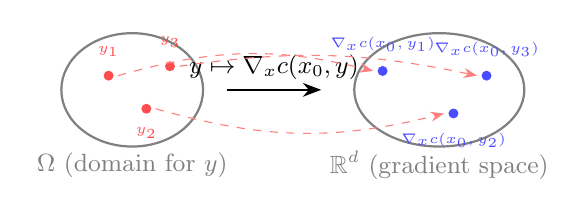
\begin{tikzpicture}[scale=0.6]
    % Domain for y
    \draw[gray, thick] (0,0) ellipse (1.5 and 1.2);
    \node[gray, font=\small] at (0, -1.6) {$\Omega$ (domain for $y$)};

    % Different y values
    \fill[red!70] (-0.5, 0.3) circle (3pt);
    \node[red!70, font=\tiny, above] at (-0.5, 0.5) {$y_1$};
    \fill[red!70] (0.3, -0.4) circle (3pt);
    \node[red!70, font=\tiny, below] at (0.3, -0.6) {$y_2$};
    \fill[red!70] (0.8, 0.5) circle (3pt);
    \node[red!70, font=\tiny, above] at (0.8, 0.7) {$y_3$};

    % Arrow to gradient space
    \draw[-{Stealth}, thick] (2, 0) -- (4, 0) node[midway, above, font=\small] {$y \mapsto \nabla_x c(x_0, y)$};

    % Gradient space
    \draw[gray, thick] (6.5,0) ellipse (1.8 and 1.2);
    \node[gray, font=\small] at (6.5, -1.6) {$\R^d$ (gradient space)};

    % Different gradients (distinct images)
    \fill[blue!70] (5.3, 0.4) circle (3pt);
    \node[blue!70, font=\tiny, above] at (5.3, 0.6) {$\nabla_x c(x_0, y_1)$};
    \fill[blue!70] (6.8, -0.5) circle (3pt);
    \node[blue!70, font=\tiny, below] at (6.8, -0.7) {$\nabla_x c(x_0, y_2)$};
    \fill[blue!70] (7.5, 0.3) circle (3pt);
    \node[blue!70, font=\tiny, above] at (7.5, 0.5) {$\nabla_x c(x_0, y_3)$};

    % Arrows connecting
    \draw[-{Stealth}, red!50, dashed] (-0.3, 0.3) to[bend left=15] (5.1, 0.4);
    \draw[-{Stealth}, red!50, dashed] (0.5, -0.4) to[bend right=15] (6.6, -0.5);
    \draw[-{Stealth}, red!50, dashed] (1, 0.5) to[bend left=10] (7.3, 0.3);
\end{tikzpicture}
\end{center}

\vspace{0.2cm}
\textbf{Consequence:} If we know $\nabla_x c(x_0, y)$, we can \textbf{uniquely recover} $y$.
\end{frame}

%==============================================================================
\begin{frame}{Why the Twist Condition?}
\textbf{Goal:} From $(x_0, y_0) \in \text{spt}(\gamma)$, deduce that $y_0$ is \textbf{uniquely determined} by $x_0$.

\vspace{0.4cm}
\textbf{Strategy:}
\begin{enumerate}
    \item From Proposition 1.15: $\nabla\phi(x_0) = \nabla_x c(x_0, y_0)$
    \item Twist condition: $y \mapsto \nabla_x c(x_0, y)$ is injective
    \item Therefore: $y_0$ is uniquely determined by $\nabla\phi(x_0)$
\end{enumerate}

\vspace{0.4cm}
\textbf{Chain of implications:}
\[
x_0 \;\xrightarrow{\nabla\phi}\; \nabla\phi(x_0) = \nabla_x c(x_0, y_0) \;\xrightarrow{\text{injectivity}}\; y_0
\]
\end{frame}

%==============================================================================
\begin{frame}{Consequence: Transport Map Exists}
From the twist condition argument:

$\Rightarrow$ $\gamma$ is concentrated on a \textbf{graph}: $\{(x, T(x))\}$

\vspace{0.3cm}
\begin{center}
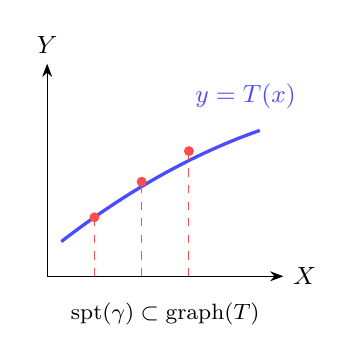
\begin{tikzpicture}[scale=0.6]
    \draw[-{Stealth}] (0,0) -- (5,0) node[right] {\small $X$};
    \draw[-{Stealth}] (0,0) -- (0,4.5) node[above] {\small $Y$};

    % Graph of T
    \draw[blue!70, very thick] plot[smooth, domain=0.3:4.5] (\x, {0.5 + 0.8*\x - 0.05*\x*\x});

    % Points with vertical lines
    \fill[red!70] (1, 1.25) circle (3pt);
    \draw[red!70, dashed] (1, 0) -- (1, 1.25);
    \fill[red!70] (2, 2) circle (3pt);
    \draw[red!70, dashed] (2, 0) -- (2, 2);
    \fill[red!70] (3, 2.65) circle (3pt);
    \draw[red!70, dashed] (3, 0) -- (3, 2.65);

    \node[blue!70, font=\small] at (4.2, 3.8) {$y = T(x)$};
    \node[font=\footnotesize] at (2.5, -0.8) {$\text{spt}(\gamma) \subset \text{graph}(T)$};
\end{tikzpicture}
\end{center}

\vspace{0.2cm}
\textbf{Key insight:} The map $T$ is constructed using $\phi$ and $c$ only, \textbf{not} $\gamma$.

$\Rightarrow$ This also gives \textbf{uniqueness} of optimal $\gamma$!
\end{frame}

%==============================================================================
\begin{frame}{Twist Condition for $c(x,y) = h(x-y)$}
For the cost $c(x,y) = h(x-y)$ with $h$ strictly convex:

\vspace{0.3cm}
\textbf{Check twist condition:}
\[
\nabla_x c(x,y) = \nabla h(x-y)
\]

The map $y \mapsto \nabla h(x_0 - y)$ is injective because:
\begin{itemize}
    \item $h$ strictly convex $\Rightarrow$ $\nabla h$ is strictly monotone
    \item $z \mapsto \nabla h(z)$ is injective
    \item $y \mapsto x_0 - y$ is bijective
\end{itemize}

\vspace{0.3cm}
\textbf{Gradient relation becomes:}
\[
\nabla\phi(x_0) = \nabla h(x_0 - y_0)
\]

\vspace{0.2cm}
\textbf{Solving for $y_0$:}
\[
\boxed{x_0 - y_0 = (\nabla h)^{-1}(\nabla\phi(x_0))}
\]

Note: $(\nabla h)^{-1}$ is well-defined for strictly convex $h$ via subdifferential theory.
\end{frame}

%==============================================================================
\section{Rademacher's Theorem}
%==============================================================================

\begin{frame}{Box 1.9: Rademacher's Theorem}
\begin{block}{Theorem (Rademacher)}
Let $f: \R^d \to \R$ be a \textbf{Lipschitz continuous} function. Then the set of points where $f$ is \textbf{not differentiable} is $\Ld$-negligible.
\end{block}

\vspace{0.3cm}
\textbf{Application to Optimal Transport:}

\begin{itemize}
    \item Kantorovich potential $\phi$ shares the same modulus of continuity as $c$
    \item For $c(x,y) = h(x-y)$ with $h$ locally Lipschitz and $\Omega$ bounded:
    \begin{itemize}
        \item $c$ is Lipschitz on $\Omega \times \Omega$
        \item $\phi$ is Lipschitz on $\Omega$
    \end{itemize}
    \item By Rademacher: $\phi$ is differentiable $\Ld$-a.e.
\end{itemize}

\vspace{0.3cm}
\textbf{Key consequence:} If $\mu \ll \Ld$ (absolutely continuous), then $\phi$ is differentiable $\mu$-a.e.

\vspace{0.2cm}
$\Rightarrow$ The formula $T(x) = x - (\nabla h)^{-1}(\nabla\phi(x))$ is valid $\mu$-a.e.!
\end{frame}

%==============================================================================
\begin{frame}{Rademacher's Theorem: Visualization}
\textbf{Lipschitz functions are ``almost everywhere smooth''}

\begin{center}
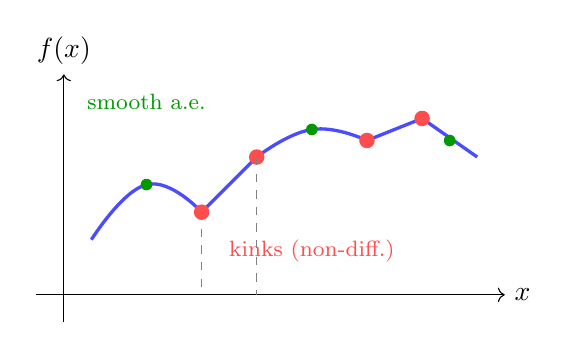
\begin{tikzpicture}[scale=0.7]
    % Axes
    \draw[->] (-0.5,0) -- (8,0) node[right] {$x$};
    \draw[->] (0,-0.5) -- (0,4) node[above] {$f(x)$};

    % Lipschitz function with kinks
    \draw[blue!70, very thick]
        plot[smooth, tension=0.8] coordinates {(0.5,1) (1.5,2) (2.5,1.5)}
        -- (3.5,2.5)  % kink
        plot[smooth, tension=0.8] coordinates {(3.5,2.5) (4.5,3) (5.5,2.8)}
        -- (6.5,3.2)  % another kink
        plot[smooth, tension=0.8] coordinates {(6.5,3.2) (7.5,2.5)};

    % Mark kinks (non-differentiable points)
    \fill[red!70] (2.5,1.5) circle (4pt);
    \fill[red!70] (3.5,2.5) circle (4pt);
    \fill[red!70] (5.5,2.8) circle (4pt);
    \fill[red!70] (6.5,3.2) circle (4pt);

    % Smooth points
    \fill[green!60!black] (1.5,2) circle (3pt);
    \fill[green!60!black] (4.5,3) circle (3pt);
    \fill[green!60!black] (7,2.8) circle (3pt);

    % Labels
    \node[red!70, font=\footnotesize] at (4.5, 0.8) {kinks (non-diff.)};
    \node[green!60!black, font=\footnotesize] at (1.5, 3.5) {smooth a.e.};

    % Annotation
    \draw[gray, dashed] (2.5, 1.5) -- (2.5, 0);
    \draw[gray, dashed] (3.5, 2.5) -- (3.5, 0);
\end{tikzpicture}
\end{center}

\vspace{0.2cm}
\textbf{Key point:} The set of ``kinks'' (non-differentiability points) has \textbf{zero measure}.

\vspace{0.2cm}
For $\phi$ Lipschitz and $\mu \ll \Ld$: $\nabla\phi$ exists $\mu$-a.e. $\Rightarrow$ transport map is well-defined!
\end{frame}

%==============================================================================
\section{Main Existence Theorem}
%==============================================================================

\begin{frame}{Theorem 1.17: Existence and Uniqueness}
\begin{block}{Theorem 1.17}
Given $\mu, \nu \in \Pp(\Omega)$ on a compact domain $\Omega \subset \R^d$, there exists an optimal transport plan $\gamma$ for the cost $c(x,y) = h(x-y)$ with $h$ strictly convex.

\vspace{0.2cm}
If $\mu$ is \textbf{absolutely continuous} and $\partial\Omega$ is $\mu$-negligible, then:
\begin{enumerate}
    \item $\gamma$ is \textbf{unique}
    \item $\gamma = (\text{id}, T)_\# \mu$ for a transport \textbf{map} $T$
    \item $T$ and the Kantorovich potential $\phi$ are linked by:
    \[
    \boxed{T(x) = x - (\nabla h)^{-1}(\nabla\phi(x))}
    \]
\end{enumerate}
\end{block}

\vspace{0.2cm}
\textbf{Key assumptions:}
\begin{itemize}
    \item $h$ strictly convex (twist condition)
    \item $\mu \ll \Ld$ (Rademacher applies)
    \item $\partial\Omega$ negligible for $\mu$
\end{itemize}
\end{frame}

%==============================================================================
\begin{frame}{Proof of Theorem 1.17}
\textbf{Step 1:} Existence of optimal $\gamma$ and $\phi$ (from previous theory).

\vspace{0.2cm}
\textbf{Step 2:} For $(x_0, y_0) \in \text{spt}(\gamma)$ with $x_0 \notin \partial\Omega$ and $\nabla\phi(x_0)$ exists:
\[
y_0 = x_0 - (\nabla h)^{-1}(\nabla\phi(x_0))
\]

\vspace{0.2cm}
\textbf{Step 3:} ``Bad'' points are $\mu$-negligible:
\begin{itemize}
    \item $\partial\Omega$ is negligible by assumption
    \item Non-differentiability points of $\phi$ are $\Ld$-negligible (Rademacher)
    \item Since $\mu \ll \Ld$, both sets are $\mu$-negligible
\end{itemize}

\vspace{0.2cm}
\textbf{Step 4:} Conclusions:
\begin{itemize}
    \item Every optimal plan is induced by a map $T$
    \item The map $T(x) = x - (\nabla h)^{-1}(\nabla\phi(x))$ is uniquely determined
    \item $\gamma = (\text{id}, T)_\# \mu$ is the unique optimal plan \hfill $\square$
\end{itemize}
\end{frame}

%==============================================================================
\begin{frame}{Proof Strategy: Flowchart}
\begin{center}
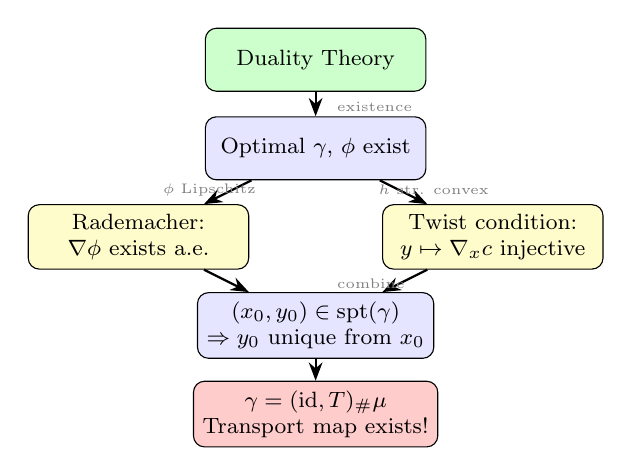
\begin{tikzpicture}[
    scale=0.75,
    box/.style={draw, rounded corners, fill=blue!10, minimum width=2.8cm, minimum height=0.8cm, font=\footnotesize, align=center},
    arrow/.style={-{Stealth}, thick},
    label/.style={font=\tiny, text=gray}
]
    % Start
    \node[box, fill=green!20] (start) at (0, 4) {Duality Theory};

    % Step 1
    \node[box] (step1) at (0, 2.5) {Optimal $\gamma$, $\phi$ exist};

    % Step 2a and 2b in parallel
    \node[box, fill=yellow!20] (step2a) at (-3, 1) {Rademacher:\\$\nabla\phi$ exists a.e.};
    \node[box, fill=yellow!20] (step2b) at (3, 1) {Twist condition:\\$y \mapsto \nabla_x c$ injective};

    % Step 3
    \node[box] (step3) at (0, -0.5) {$(x_0, y_0) \in \text{spt}(\gamma)$\\$\Rightarrow y_0$ unique from $x_0$};

    % Step 4
    \node[box, fill=red!20] (step4) at (0, -2) {$\gamma = (\text{id}, T)_\#\mu$\\Transport map exists!};

    % Arrows
    \draw[arrow] (start) -- (step1);
    \draw[arrow] (step1) -- (step2a);
    \draw[arrow] (step1) -- (step2b);
    \draw[arrow] (step2a) -- (step3);
    \draw[arrow] (step2b) -- (step3);
    \draw[arrow] (step3) -- (step4);

    % Labels on arrows
    \node[label, right] at (0.2, 3.2) {existence};
    \node[label] at (-1.8, 1.8) {$\phi$ Lipschitz};
    \node[label] at (2, 1.8) {$h$ str. convex};
    \node[label, right] at (0.2, 0.2) {combine};
\end{tikzpicture}
\end{center}

\textbf{Key ingredients:} Duality $+$ Rademacher $+$ Twist condition $\Rightarrow$ Optimal map!
\end{frame}

%==============================================================================
\begin{frame}{Visualization: Optimal Transport Map}
\begin{columns}
\begin{column}{0.5\textwidth}
\textbf{The optimal map formula:}
\[
T(x) = x - (\nabla h)^{-1}(\nabla\phi(x))
\]

\vspace{0.3cm}
\textbf{Interpretation:}
\begin{itemize}
    \item $\nabla\phi(x)$: direction from potential
    \item $(\nabla h)^{-1}$: invert the cost structure
    \item $x - \cdot$: displacement from $x$
\end{itemize}

\vspace{0.3cm}
\textbf{Special case $h(z) = \frac{1}{2}|z|^2$:}
\[
\nabla h(z) = z, \quad (\nabla h)^{-1} = \text{id}
\]
\[
T(x) = x - \nabla\phi(x)
\]
\end{column}
\begin{column}{0.5\textwidth}
\begin{center}
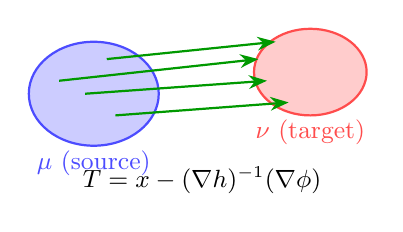
\begin{tikzpicture}[scale=0.55]
    % Source region
    \fill[blue!20] (0,0) ellipse (1.5 and 1.2);
    \draw[blue!70, thick] (0,0) ellipse (1.5 and 1.2);
    \node[blue!70, font=\small] at (0, -1.6) {$\mu$ (source)};

    % Target region
    \fill[red!20] (5,0.5) ellipse (1.3 and 1);
    \draw[red!70, thick] (5,0.5) ellipse (1.3 and 1);
    \node[red!70, font=\small] at (5, -0.9) {$\nu$ (target)};

    % Transport arrows
    \draw[-{Stealth}, thick, green!60!black] (0.3, 0.8) -- (4.2, 1.2);
    \draw[-{Stealth}, thick, green!60!black] (-0.2, 0) -- (4, 0.3);
    \draw[-{Stealth}, thick, green!60!black] (0.5, -0.5) -- (4.5, -0.2);
    \draw[-{Stealth}, thick, green!60!black] (-0.8, 0.3) -- (3.8, 0.8);

    \node[font=\small] at (2.5, -2) {$T = x - (\nabla h)^{-1}(\nabla\phi)$};
\end{tikzpicture}

\vspace{0.3cm}
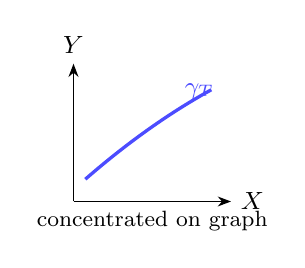
\begin{tikzpicture}[scale=0.5]
    % Graph representation
    \draw[-{Stealth}] (0,0) -- (4,0) node[right] {\small $X$};
    \draw[-{Stealth}] (0,0) -- (0,3.5) node[above] {\small $Y$};

    % Graph of T
    \draw[blue!70, very thick] plot[smooth, domain=0.3:3.5] (\x, {0.3 + 0.9*\x - 0.05*\x*\x});

    \node[blue!70, font=\small] at (3.2, 2.8) {$\gamma_T$};
    \node[font=\footnotesize] at (2, -0.5) {concentrated on graph};
\end{tikzpicture}
\end{center}
\end{column}
\end{columns}
\end{frame}

%==============================================================================
\section{Important Remarks}
%==============================================================================

\begin{frame}{Remark 1.18: $p$-Costs}
\begin{block}{Remark 1.18}
All costs of the form $c(x,y) = |x-y|^p$ with $p > 1$ can be handled via Theorem 1.17.
\end{block}

\vspace{0.3cm}
\textbf{Verification:} $h(z) = |z|^p$ is strictly convex for $p > 1$.

\vspace{0.3cm}
\begin{center}
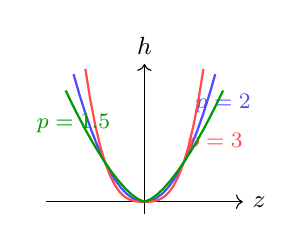
\begin{tikzpicture}[scale=0.5]
    \draw[->] (-2.5,0) -- (2.5,0) node[right] {\small $z$};
    \draw[->] (0,-0.3) -- (0,3.5) node[above] {\small $h$};

    % p = 2
    \draw[blue!70, thick, domain=-1.8:1.8] plot (\x, {\x*\x});
    \node[blue!70, font=\footnotesize] at (2, 2.5) {$p=2$};

    % p = 3
    \draw[red!70, thick, domain=-1.5:1.5] plot (\x, {abs(\x)^3});
    \node[red!70, font=\footnotesize] at (1.8, 1.5) {$p=3$};

    % p = 1.5
    \draw[green!60!black, thick, domain=-2:2] plot (\x, {abs(\x)^1.5});
    \node[green!60!black, font=\footnotesize] at (-1.8, 2) {$p=1.5$};
\end{tikzpicture}
\end{center}

\vspace{0.2cm}
\textbf{Note:} The case $p = 1$ (Monge's original cost) is \textbf{not} covered---$h(z) = |z|$ is convex but not strictly convex.
\end{frame}

%==============================================================================
\begin{frame}{Remark 1.19: Uniqueness via Convexity}
\begin{block}{Remark 1.19}
When any optimal $\gamma$ must be induced by a map $T$, we have \textbf{uniqueness}.
\end{block}

\vspace{0.3cm}
\textbf{Proof:} Suppose $\gamma_1 = \gamma_{T_1}$ and $\gamma_2 = \gamma_{T_2}$ are both optimal.

\vspace{0.2cm}
Then $\frac{1}{2}\gamma_1 + \frac{1}{2}\gamma_2$ is also optimal (by convexity of (KP)).

\vspace{0.2cm}
But this plan cannot be induced by a map unless $T_1 = T_2$ $\mu$-a.e.

\vspace{0.2cm}
$\Rightarrow$ Contradiction unless $\gamma_1 = \gamma_2$.

\vspace{0.4cm}
\begin{center}
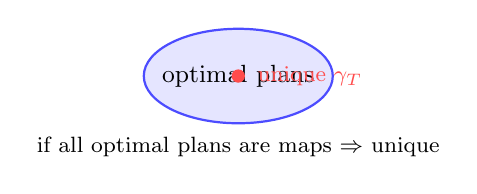
\begin{tikzpicture}[scale=0.6]
    % Convex set of optimal plans
    \draw[blue!70, thick, fill=blue!10] (0,0) ellipse (2 and 1);
    \node[font=\small] at (0, 0) {optimal plans};

    % Unique point
    \fill[red!70] (0, 0) circle (4pt);
    \node[red!70, right, font=\footnotesize] at (0.2, 0) {unique $\gamma_T$};

    \node[font=\footnotesize] at (0, -1.5) {if all optimal plans are maps $\Rightarrow$ unique};
\end{tikzpicture}
\end{center}
\end{frame}

%==============================================================================
\begin{frame}{Remark 1.20: Invertibility of $T$}
\begin{block}{Remark 1.20}
If both $\mu$ and $\nu$ satisfy the assumptions of Theorem 1.17, then there exist optimal maps in \textbf{both directions}:
\[
\gamma = (\text{id}, T)_\# \mu = (S, \text{id})_\# \nu
\]
\end{block}

\vspace{0.3cm}
\textbf{Consequence:}
\begin{itemize}
    \item $\gamma$-a.e.: $y = T(x)$ and $x = S(y)$
    \item This means: $S(T(x)) = x$ for $\mu$-a.e. $x$
    \item $T$ is \textbf{invertible} on a set of full measure
    \item $T^{-1} = S$ is the optimal map from $\nu$ to $\mu$
\end{itemize}

\vspace{0.3cm}
\begin{center}
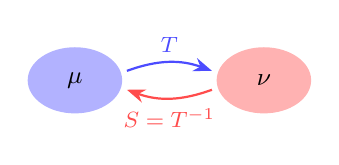
\begin{tikzpicture}[scale=0.6]
    \fill[blue!30] (0,0) ellipse (1 and 0.7);
    \node[font=\small] at (0, 0) {$\mu$};

    \fill[red!30] (4,0) ellipse (1 and 0.7);
    \node[font=\small] at (4, 0) {$\nu$};

    \draw[-{Stealth}, thick, blue!70] (1.1, 0.2) to[bend left=20] node[above, font=\footnotesize] {$T$} (2.9, 0.2);
    \draw[-{Stealth}, thick, red!70] (2.9, -0.2) to[bend left=20] node[below, font=\footnotesize] {$S = T^{-1}$} (1.1, -0.2);
\end{tikzpicture}
\end{center}
\end{frame}

%==============================================================================
\section{The Quadratic Case}
%==============================================================================

\begin{frame}{Section 1.3.1: The Quadratic Case in $\R^d$}
The case $c(x,y) = \frac{1}{2}|x-y|^2$ deserves special attention.

\vspace{0.3cm}
\textbf{Key connection:} $c$-concavity $\Leftrightarrow$ classical convexity!

\vspace{0.3cm}
\begin{block}{Proposition 1.21}
Given $\chi: \R^d \to \R \cup \{-\infty\}$, define $u_\chi(x) = \frac{1}{2}|x|^2 - \chi(x)$.

Then:
\[
\boxed{u_{\chi^c} = (u_\chi)^*}
\]
where $(u_\chi)^*$ is the \textbf{Legendre transform} (convex conjugate).

\vspace{0.2cm}
In particular: $\zeta$ is $c$-concave $\Leftrightarrow$ $\frac{1}{2}|x|^2 - \zeta(x)$ is convex and l.s.c.
\end{block}
\end{frame}

%==============================================================================
\begin{frame}{Proof of Proposition 1.21: Computation}
\textbf{Goal:} Show $u_{\chi^c} = (u_\chi)^*$ where $u_\chi(x) = \frac{1}{2}|x|^2 - \chi(x)$.

\vspace{0.3cm}
\textbf{Step 1:} Expand using definition of $c$-transform:
\begin{align*}
u_{\chi^c}(x) &= \frac{1}{2}|x|^2 - \chi^c(x) \\
&= \frac{1}{2}|x|^2 - \inf_y \left[\frac{1}{2}|x-y|^2 - \chi(y)\right]
\end{align*}

\vspace{0.2cm}
\textbf{Step 2:} Convert inf to sup:
\[
= \sup_y \left[\frac{1}{2}|x|^2 - \frac{1}{2}|x-y|^2 + \chi(y)\right]
\]
\end{frame}

%==============================================================================
\begin{frame}{Proof of Proposition 1.21: Conclusion}
\textbf{Step 3:} Simplify using $|x|^2 - |x-y|^2 = 2x \cdot y - |y|^2$:
\begin{align*}
u_{\chi^c}(x) &= \sup_y \left[x \cdot y - \frac{1}{2}|y|^2 + \chi(y)\right] \\
&= \sup_y \left[x \cdot y - \underbrace{\left(\frac{1}{2}|y|^2 - \chi(y)\right)}_{= u_\chi(y)}\right] \\
&= (u_\chi)^*(x) \quad \checkmark
\end{align*}

\vspace{0.3cm}
\textbf{Second part:}
\begin{itemize}
    \item $c$-concave functions are $c$-transforms
    \item Convex l.s.c. functions are Legendre transforms
    \item The correspondence $\chi \leftrightarrow u_\chi$ links these \hfill $\square$
\end{itemize}
\end{frame}

%==============================================================================
\begin{frame}{Brenier's Theorem}
\textbf{Consequence of Proposition 1.21:}

For $c(x,y) = \frac{1}{2}|x-y|^2$, the optimal map is:
\[
T(x) = x - \nabla\phi(x) = \nabla\left(\frac{|x|^2}{2} - \phi(x)\right) = \nabla u(x)
\]
where $u$ is a \textbf{convex function}.

\vspace{0.3cm}
\begin{block}{Brenier's Theorem (1991)}
If $\mu \ll \Ld$, then there exists a \textbf{unique} optimal transport map $T$ from $\mu$ to $\nu$ for the quadratic cost, and:
\[
\boxed{T = \nabla u \quad \text{for a convex function } u}
\]
\end{block}

\vspace{0.3cm}
\textbf{Historical note:} This is one of the most celebrated results in optimal transport theory. Section 1.7.2 presents Brenier's original ``polar factorization'' approach.
\end{frame}

%==============================================================================
\begin{frame}{The Magic of Quadratic Cost: $c$-Concavity $\Leftrightarrow$ Convexity}
\textbf{Key correspondence for $c(x,y) = \frac{1}{2}|x-y|^2$:}

\begin{center}
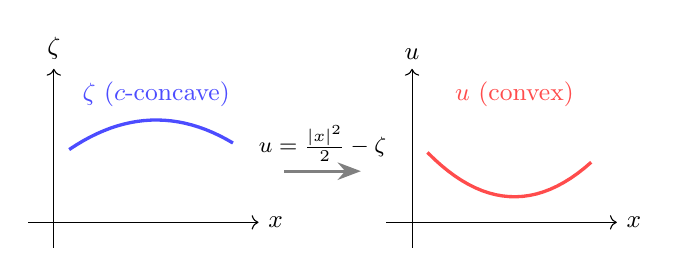
\begin{tikzpicture}[scale=0.65]
    % Left side: c-concave function
    \draw[->] (-0.5,0) -- (4,0) node[right] {\small $x$};
    \draw[->] (0,-0.5) -- (0,3) node[above] {\small $\zeta$};

    % c-concave function (concave-looking)
    \draw[blue!70, very thick, domain=0.3:3.5] plot (\x, {2 - 0.2*(\x-2)^2});
    \node[blue!70, font=\small] at (2, 2.5) {$\zeta$ ($c$-concave)};

    % Arrow
    \draw[-{Stealth}, very thick, gray] (4.5, 1) -- (6, 1);
    \node[above, font=\footnotesize] at (5.25, 1) {$u = \frac{|x|^2}{2} - \zeta$};

    % Right side: convex function
    \begin{scope}[shift={(7,0)}]
        \draw[->] (-0.5,0) -- (4,0) node[right] {\small $x$};
        \draw[->] (0,-0.5) -- (0,3) node[above] {\small $u$};

        % convex function
        \draw[red!70, very thick, domain=0.3:3.5] plot (\x, {0.3*(\x-2)^2 + 0.5});
        \node[red!70, font=\small] at (2, 2.5) {$u$ (convex)};
    \end{scope}
\end{tikzpicture}
\end{center}

\vspace{0.2cm}
\textbf{Why this matters:}
\begin{itemize}
    \item Kantorovich potential $\phi$ is $c$-concave
    \item Therefore $u = \frac{|x|^2}{2} - \phi$ is convex
    \item Optimal map $T = x - \nabla\phi = \nabla u$ is gradient of convex function!
\end{itemize}

\textbf{Convex analysis tools become available} (subdifferentials, Legendre transforms, etc.)
\end{frame}

%==============================================================================
\begin{frame}{Visualization: Gradient of Convex Function}
\begin{columns}
\begin{column}{0.5\textwidth}
\textbf{Brenier's result:}
\[
T = \nabla u, \quad u \text{ convex}
\]

\vspace{0.2cm}
\textbf{Properties of $\nabla u$:}
\begin{itemize}
    \item Monotone (in the sense of operators)
    \item Maps level sets of $u$ to regions
    \item Preserves certain geometric structures
\end{itemize}

\vspace{0.3cm}
\textbf{Connection to Monge-Amp\`ere:}
\[
\det(D^2 u) = \frac{f}{g \circ \nabla u}
\]
where $\mu = f \cdot \Ld$, $\nu = g \cdot \Ld$.
\end{column}
\begin{column}{0.5\textwidth}
\begin{center}
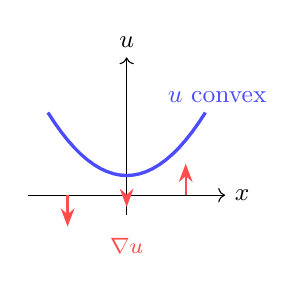
\begin{tikzpicture}[scale=0.5]
    % Convex function
    \draw[->] (-2.5,0) -- (2.5,0) node[right] {\small $x$};
    \draw[->] (0,-0.5) -- (0,3.5) node[above] {\small $u$};

    \draw[blue!70, very thick, domain=-2:2] plot (\x, {0.4*\x*\x + 0.5});
    \node[blue!70, font=\small] at (2.3, 2.5) {$u$ convex};

    % Gradient arrows
    \draw[-{Stealth}, red!70, thick] (-1.5, 0) -- (-1.5, -0.8);
    \draw[-{Stealth}, red!70, thick] (0, 0) -- (0, -0.3);
    \draw[-{Stealth}, red!70, thick] (1.5, 0) -- (1.5, 0.8);

    \node[red!70, font=\footnotesize] at (0, -1.3) {$\nabla u$};
\end{tikzpicture}

\vspace{0.3cm}
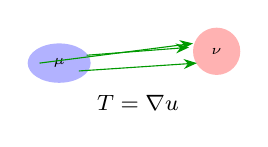
\begin{tikzpicture}[scale=0.5]
    % Transport visualization
    \fill[blue!30] (-2, 0) ellipse (0.8 and 0.5);
    \node[font=\tiny] at (-2, 0) {$\mu$};

    \fill[red!30] (2, 0.3) ellipse (0.6 and 0.6);
    \node[font=\tiny] at (2, 0.3) {$\nu$};

    % Arrows showing T = nabla u
    \draw[-{Stealth}, green!60!black] (-1.3, 0.2) -- (1.3, 0.4);
    \draw[-{Stealth}, green!60!black] (-1.5, -0.2) -- (1.5, 0);
    \draw[-{Stealth}, green!60!black] (-2.5, 0) -- (1.4, 0.5);

    \node[font=\footnotesize] at (0, -1) {$T = \nabla u$};
\end{tikzpicture}
\end{center}
\end{column}
\end{columns}
\end{frame}

%==============================================================================
\section{Unbounded Domains}
%==============================================================================

\begin{frame}{Theorem 1.22: Unbounded Domains}
\begin{block}{Theorem 1.22}
Let $\mu, \nu \in \Pp(\R^d)$ and $c(x,y) = \frac{1}{2}|x-y|^2$. Suppose:
\begin{enumerate}
    \item $\int |x|^2 \, d\mu, \int |y|^2 \, d\nu < +\infty$ (finite second moments)
    \item $\mu$ gives no mass to $(d-1)$-surfaces of class $C^2$
\end{enumerate}
Then there exists a \textbf{unique} optimal transport map $T$ from $\mu$ to $\nu$, and $T = \nabla u$ for a convex function $u$.
\end{block}

\vspace{0.3cm}
\textbf{Key tool:} Use the variant dual problem (DP-var):
\[
\text{(DP-var)} \quad \sup\left\{\int_{\R^d} \phi \, d\mu + \int_{\R^d} \psi \, d\nu : \phi \in L^1(\mu), \psi \in L^1(\nu), \phi \oplus \psi \leq c\right\}
\]

\vspace{0.2cm}
\textbf{Result:} $\max(\text{DP-var}) = \min(\text{KP})$ without compactness!
\end{frame}

%==============================================================================
\begin{frame}{Proof Sketch of Theorem 1.22}
\textbf{Step 1:} Existence of optimal $\gamma$ and dual pair $(\phi, \psi) \in L^1(\mu) \times L^1(\nu)$.

\vspace{0.2cm}
\textbf{Step 2:} $\gamma$ concentrated on graph of $T(x) = x - \nabla\phi(x) = \nabla u(x)$ where differentiable.

\vspace{0.2cm}
\textbf{Step 3:} Handle non-differentiability:
\begin{itemize}
    \item Since $\phi \in L^1(\mu)$, we have $u$ finite $\mu$-a.e.
    \item $\text{spt}(\mu) \subset \{u < +\infty\}$ (a convex set)
    \item $\partial\{u < +\infty\}$ is $(d-1)$-$C^2$ rectifiable, hence $\mu$-negligible
    \item In interior of $\{u < +\infty\}$, $u$ differentiable $\mu$-a.e.
\end{itemize}

\vspace{0.2cm}
\textbf{Conclusion:} Same result as compact case. \hfill $\square$

\vspace{0.3cm}
\textbf{Footnote (Gigli):} The condition ``$\mu(A) = 0$ for every $C^2$ surface $A$ of co-dimension 1'' \textbf{characterizes} measures for which optimal transport is unique and induced by a map, for any target $\nu$.
\end{frame}

%==============================================================================
\section{One-Dimensional Case}
%==============================================================================

\begin{frame}{Remark 1.23: Dimension One}
\begin{block}{Remark 1.23}
In dimension $d = 1$, if $\mu \in \Pp(\R)$ is \textbf{atomless} (no point masses), then an optimal transport map exists for the quadratic cost, for any target $\nu$.
\end{block}

\vspace{0.3cm}
\textbf{Why?}
\begin{itemize}
    \item Non-differentiability points of a convex function in 1D are \textbf{at most countable}
    \item Atomless $\mu$ gives zero mass to countable sets
    \item Hence differentiability holds $\mu$-a.e.
\end{itemize}

\vspace{0.3cm}
\textbf{Form of optimal map:}
\[
T = u' \quad \text{where } u \text{ convex}
\]
$\Rightarrow$ $T$ is \textbf{non-decreasing}!

\vspace{0.3cm}
\textbf{Connection to quantile functions:} $T = F_\nu^{-1} \circ F_\mu$ (monotone rearrangement).
\end{frame}

%==============================================================================
\begin{frame}{1D Optimal Transport Visualization}
\begin{columns}
\begin{column}{0.5\textwidth}
\textbf{In 1D:} Optimal map is monotone.

\vspace{0.2cm}
\textbf{Quantile formula:}
\[
T(x) = F_\nu^{-1}(F_\mu(x))
\]
where $F_\mu, F_\nu$ are CDFs.

\vspace{0.3cm}
\textbf{Interpretation:}
\begin{itemize}
    \item Map $p$-th quantile of $\mu$ to $p$-th quantile of $\nu$
    \item Preserves order
    \item $T = \nabla u$ with $u$ convex
\end{itemize}

\vspace{0.2cm}
\textbf{Key insight:} In 1D, optimal transport has an \textbf{explicit formula}!
\end{column}
\begin{column}{0.5\textwidth}
\begin{center}
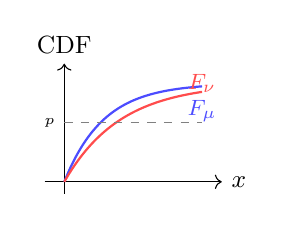
\begin{tikzpicture}[scale=0.5]
    % CDFs
    \draw[->] (-0.5,0) -- (4,0) node[right] {\small $x$};
    \draw[->] (0,-0.3) -- (0,3) node[above] {\small CDF};

    \draw[blue!70, thick] plot[smooth, domain=0:3.5] (\x, {2.5*(1-exp(-\x))});
    \node[blue!70, font=\footnotesize] at (3.5, 1.8) {$F_\mu$};

    \draw[red!70, thick] plot[smooth, domain=0:3.5] (\x, {2.5*(1-exp(-0.7*\x))});
    \node[red!70, font=\footnotesize] at (3.5, 2.5) {$F_\nu$};

    % Horizontal line at p
    \draw[gray, dashed] (0, 1.5) -- (3.5, 1.5);
    \node[left, font=\tiny] at (0, 1.5) {$p$};
\end{tikzpicture}

\vspace{0.2cm}
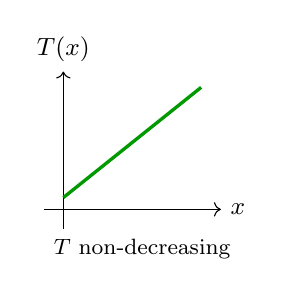
\begin{tikzpicture}[scale=0.5]
    % Monotone map
    \draw[->] (-0.5,0) -- (4,0) node[right] {\small $x$};
    \draw[->] (0,-0.5) -- (0,3.5) node[above] {\small $T(x)$};

    \draw[green!60!black, very thick] plot[smooth, domain=0:3.5] (\x, {0.3 + 0.8*\x});

    \node[font=\footnotesize] at (2, -1) {$T$ non-decreasing};
\end{tikzpicture}

\vspace{0.2cm}
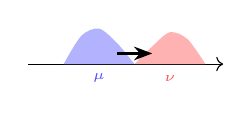
\begin{tikzpicture}[scale=0.45]
    % Real line transport
    \draw[->] (-0.5,0) -- (5,0);

    % Source density
    \fill[blue!30] plot[smooth] coordinates {(0.5,0) (1,0.8) (1.5,1) (2,0.6) (2.5,0)} -- cycle;
    \node[blue!70, font=\tiny] at (1.5, -0.4) {$\mu$};

    % Target density
    \fill[red!30] plot[smooth] coordinates {(2.5,0) (3,0.5) (3.5,0.9) (4,0.7) (4.5,0)} -- cycle;
    \node[red!70, font=\tiny] at (3.5, -0.4) {$\nu$};

    % Arrow
    \draw[-{Stealth}, thick] (2, 0.3) -- (3, 0.3);
\end{tikzpicture}
\end{center}
\end{column}
\end{columns}
\end{frame}

%==============================================================================
\begin{frame}{Monotone Rearrangement: Why It Works}
\textbf{Intuition:} In 1D, the optimal map ``rearranges'' mass in order-preserving way.

\begin{center}
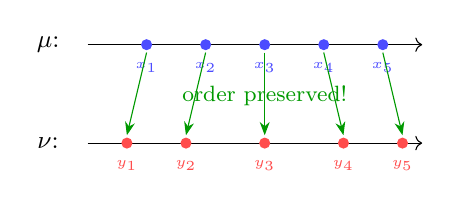
\begin{tikzpicture}[scale=0.5]
    % Source distribution
    \draw[->] (-0.5, 2.5) -- (8, 2.5);
    \node[font=\small] at (-1.5, 2.5) {$\mu$:};

    % Source points
    \foreach \x/\lab in {1/x_1, 2.5/x_2, 4/x_3, 5.5/x_4, 7/x_5} {
        \fill[blue!70] (\x, 2.5) circle (4pt);
        \node[below, font=\tiny, blue!70] at (\x, 2.3) {$\lab$};
    }

    % Target distribution
    \draw[->] (-0.5, 0) -- (8, 0);
    \node[font=\small] at (-1.5, 0) {$\nu$:};

    % Target points (stretched out)
    \foreach \x/\lab in {0.5/y_1, 2/y_2, 4/y_3, 6/y_4, 7.5/y_5} {
        \fill[red!70] (\x, 0) circle (4pt);
        \node[below, font=\tiny, red!70] at (\x, -0.2) {$\lab$};
    }

    % Monotone matching arrows
    \draw[-{Stealth}, green!60!black] (1, 2.3) -- (0.5, 0.2);
    \draw[-{Stealth}, green!60!black] (2.5, 2.3) -- (2, 0.2);
    \draw[-{Stealth}, green!60!black] (4, 2.3) -- (4, 0.2);
    \draw[-{Stealth}, green!60!black] (5.5, 2.3) -- (6, 0.2);
    \draw[-{Stealth}, green!60!black] (7, 2.3) -- (7.5, 0.2);

    % Label
    \node[green!60!black, font=\footnotesize] at (4, 1.2) {order preserved!};
\end{tikzpicture}
\end{center}

\vspace{0.2cm}
\textbf{Why monotone is optimal:}
\begin{itemize}
    \item Any ``crossing'' transport $x_1 < x_2$, $T(x_1) > T(x_2)$ can be improved
    \item Uncrossing reduces total cost (triangle inequality argument)
    \item Monotone map = unique optimal for $c(x,y) = h(x-y)$, $h$ convex
\end{itemize}

\textbf{Explicit formula:} $T = F_\nu^{-1} \circ F_\mu$ (quantile matching)
\end{frame}

%==============================================================================
\begin{frame}{Remark 1.24: General $C^{1,1}$ Costs}
\begin{block}{Remark 1.24}
Properties of the quadratic case extend to general costs $c(x,y)$ that are $C^{1,1}$ and satisfy the twist condition (Definition 1.16).
\end{block}

\vspace{0.3cm}
\textbf{Key observation:} The transport map is no longer the gradient of a convex function, but the Kantorovich potential $\phi$ is \textbf{semi-concave}.

\vspace{0.3cm}
\textbf{Semi-concavity:} $\phi$ is concave up to subtracting a quadratic function:
\[
x \mapsto \phi(x) - C|x|^2 \quad \text{is concave for some } C > 0
\]

\vspace{0.3cm}
\textbf{Consequence:}
\begin{itemize}
    \item Semi-concave functions have similar differentiability properties as convex functions
    \item Same assumptions on $\mu$ as in Theorem 1.22 work
    \item Non-differentiability set is $(d-1)$-rectifiable
\end{itemize}
\end{frame}

%==============================================================================
\section{The Flat Torus}
%==============================================================================

\begin{frame}{Section 1.3.2: Quadratic Cost on the Flat Torus}
\textbf{Setting:} Flat torus $\Td = \R^d / \Z^d$, cost:
\[
c(x,y) = \frac{1}{2}|[x-y]|^2
\]
where the \textbf{periodic distance} is:
\[
\boxed{|[z]| := \min\{|z + k| : k \in \Z^d\}}
\]

\vspace{0.3cm}
\textbf{Why study the torus?}
\begin{itemize}
    \item Simplest example of OT on a manifold
    \item No boundary issues
    \item Compactly supported measures on $\R^d$ can be viewed on a large torus
    \item If supports are far from boundary, results match $\R^d$ case
\end{itemize}

\vspace{0.2cm}
\textbf{Reference:} First studied in [128], general manifold case by McCann [231].
\end{frame}

%==============================================================================
\begin{frame}{Properties of Periodic Distance}
\textbf{For $z \in Q := [-\frac{1}{2}, \frac{1}{2}]^d$:}
\begin{itemize}
    \item Optimal $\bar{k} \in \{-1, 0, +1\}^d$ achieving $|[z]| = |z + \bar{k}|$
    \item $\bar{k}$ is unique (and equals $0$) unless $z \in \partial Q$
\end{itemize}

\vspace{0.4cm}
\textbf{Semi-concavity:}

The function $z \mapsto \frac{1}{2}|[z]|^2$ is \textbf{semi-concave}:
\[
\frac{1}{2}|[z]|^2 = \inf_{k \in \Z^d} \frac{1}{2}|z + k|^2
\]
(infimum of quadratics with Hessian $= I$)

\vspace{0.3cm}
\textbf{Consequence:} Differentiable everywhere except on $\partial Q + \Z^d$.
\end{frame}

%==============================================================================
\begin{frame}{Cutlocus on the Torus}
\begin{block}{Definition (Cutlocus)}
For a point $x$, the \textbf{cutlocus} of $x$ is:
\[
\text{cut}(x) = \{y : \text{squared distance is not differentiable at } (x,y)\}
\]
On $\Td$: $\text{cut}(x) = \{y : y - x \in \partial Q + \Z^d\}$
\end{block}

\vspace{0.2cm}
\begin{center}
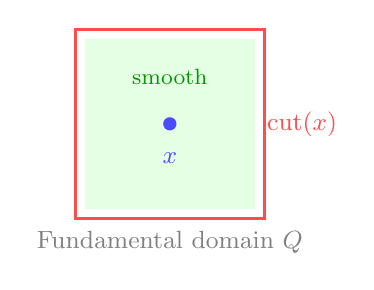
\begin{tikzpicture}[scale=0.6]
    % Torus fundamental domain
    \draw[gray, thick] (-2,-2) rectangle (2,2);
    \node[gray, font=\small] at (0, -2.5) {Fundamental domain $Q$};

    % Interior (smooth region)
    \fill[green!20, opacity=0.5] (-1.8,-1.8) rectangle (1.8,1.8);

    % Cut locus (boundary)
    \draw[red!70, very thick] (-2,-2) rectangle (2,2);

    % Point x at origin
    \fill[blue!70] (0,0) circle (4pt);
    \node[below, blue!70, font=\small] at (0, -0.4) {$x$};

    % Labels
    \node[red!70, font=\small] at (2.8, 0) {cut$(x)$};
    \node[green!60!black, font=\footnotesize] at (0, 1) {smooth};
\end{tikzpicture}
\end{center}

\textbf{Intuition:} At the cutlocus, there are multiple shortest paths from $x$ to $y$.
\end{frame}

%==============================================================================
\begin{frame}{Theorem 1.25: Existence on the Torus}
\begin{block}{Theorem 1.25}
Take $\mu, \nu \in \Pp(\Td)$ with $\mu \ll \Ld$ and $c(x,y) = \frac{1}{2}|[x-y]|^2$.

Then there exists a \textbf{unique} optimal transport plan $\gamma \in \Pi(\mu, \nu)$. It has the form $\gamma = \gamma_T$ and the optimal map is:
\[
\boxed{T(x) = x - \nabla\phi(x) \mod \Z^d}
\]
where $\phi$ is a Kantorovich potential. Moreover, for a.e. $x \in \Td$:
\[
T(x) \notin \text{cut}(x)
\]
\end{block}

\vspace{0.3cm}
\textbf{Key point:} The proof follows the same strategy as for $h(x-y)$ costs, using semi-concavity of $\phi$ and the twist condition.
\end{frame}

%==============================================================================
\begin{frame}{Torus Transport: Visualization}
\begin{center}
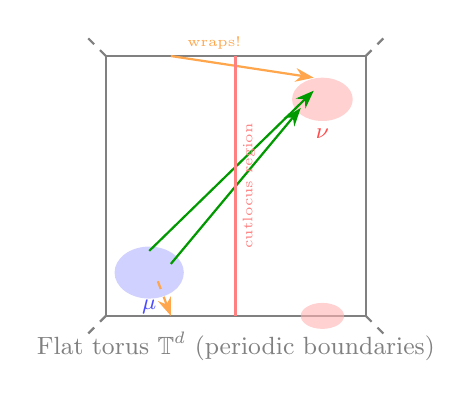
\begin{tikzpicture}[scale=0.55]
    % Flat torus as square with periodic boundaries
    \draw[gray, thick] (0,0) rectangle (6,6);

    % Periodic boundary indicators
    \draw[gray, thick, dashed] (0,0) -- (-0.5,-0.5);
    \draw[gray, thick, dashed] (6,0) -- (6.5,-0.5);
    \draw[gray, thick, dashed] (0,6) -- (-0.5,6.5);
    \draw[gray, thick, dashed] (6,6) -- (6.5,6.5);

    % Label
    \node[gray, font=\small] at (3, -0.7) {Flat torus $\Td$ (periodic boundaries)};

    % Source distribution (blue region)
    \fill[blue!30, opacity=0.6] (1,1) ellipse (0.8 and 0.6);
    \node[blue!70, font=\footnotesize] at (1, 0.2) {$\mu$};

    % Target distribution (red region, split across boundary!)
    \fill[red!30, opacity=0.6] (5,5) ellipse (0.7 and 0.5);
    \fill[red!30, opacity=0.6] (5,0) ellipse (0.5 and 0.3);  % wraps to bottom
    \node[red!70, font=\footnotesize] at (5, 4.2) {$\nu$};

    % Transport arrows (some wrap around)
    \draw[-{Stealth}, green!60!black, thick] (1.5, 1.2) -- (4.5, 4.8);
    \draw[-{Stealth}, green!60!black, thick] (1, 1.5) -- (4.8, 5.2);

    % Wrapping transport (goes through top, appears at bottom)
    \draw[-{Stealth}, orange!70, thick, dashed] (1.2, 0.8) -- (1.5, 0);
    \draw[-{Stealth}, orange!70, thick] (1.5, 6) -- (4.8, 5.5);
    \node[orange!70, font=\tiny] at (2.5, 6.3) {wraps!};

    % Cutlocus indication
    \draw[red!50, very thick] (3, 0) -- (3, 6);
    \node[red!50, font=\tiny, rotate=90] at (3.3, 3) {cutlocus region};
\end{tikzpicture}
\end{center}

\textbf{Key features on torus:}
\begin{itemize}
    \item Transport can ``wrap around'' periodic boundaries
    \item Cutlocus: where multiple shortest paths exist
    \item Theorem 1.25: optimal $T(x)$ avoids cutlocus a.e.
\end{itemize}
\end{frame}

%==============================================================================
\begin{frame}{Proof Sketch of Theorem 1.25}
\textbf{Setup:} Take optimal $\gamma$ and dual pair $(\phi, \psi)$. Fix $(x_0, y_0) \in \text{spt}(\gamma)$.

\vspace{0.2cm}
\textbf{Key inequalities:}
\[
\frac{1}{2}|[x - y_0]|^2 - \phi(x) \geq \psi(y_0), \quad \frac{1}{2}|[x_0 - y_0]|^2 - \phi(x_0) = \psi(y_0)
\]

\vspace{0.2cm}
\textbf{Choose $k_0 \in \Z^d$} such that $|[x_0 - y_0]| = |x_0 - y_0 - k_0|$.

Then: $x \mapsto \frac{1}{2}|x - y_0 - k_0|^2 - \phi(x)$ is minimal at $x = x_0$.

\vspace{0.2cm}
\textbf{Semi-concavity:} $\phi(x) = \inf_y \frac{1}{2}|[x-y]|^2 - \psi(y)$ is semi-concave, hence differentiable $\mu$-a.e.

\vspace{0.2cm}
\textbf{If $\nabla\phi(x_0)$ exists:}
\[
x_0 - y_0 - k_0 = \nabla\phi(x_0) \quad \Rightarrow \quad k_0 \text{ unique}, \; y_0 \notin \text{cut}(x_0)
\]

$\Rightarrow$ $y_0$ uniquely determined $\Rightarrow$ existence and uniqueness of $T$. \hfill $\square$
\end{frame}

%==============================================================================
\begin{frame}{Remark 1.26: Connection to $\R^d$}
\begin{block}{Remark 1.26}
If $\text{spt}(\mu), \text{spt}(\nu) \subset \frac{1}{2}Q$, then the transport on $\Td$ is \textbf{identical} to the classical quadratic transport on $\R^d$.
\end{block}

\vspace{0.3cm}
\textbf{Why?} In the proof, we have $k_0 = 0$ when $x_0 - y_0 \in Q$.

If both supports are in $\frac{1}{2}Q$, then all differences $x - y$ lie in $Q$, so $k_0 = 0$ always.

\vspace{0.4cm}
\begin{center}
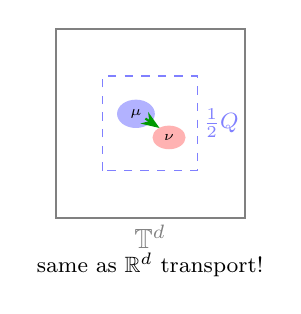
\begin{tikzpicture}[scale=0.6]
    % Torus
    \draw[gray, thick] (-2,-2) rectangle (2,2);
    \node[gray] at (0, -2.4) {$\Td$};

    % Half Q
    \draw[blue!50, dashed] (-1,-1) rectangle (1,1);
    \node[blue!50, font=\footnotesize] at (1.5, 0) {$\frac{1}{2}Q$};

    % Supports
    \fill[blue!30] (-0.3, 0.2) ellipse (0.4 and 0.3);
    \node[font=\tiny] at (-0.3, 0.2) {$\mu$};

    \fill[red!30] (0.4, -0.3) ellipse (0.35 and 0.25);
    \node[font=\tiny] at (0.4, -0.3) {$\nu$};

    % Arrow
    \draw[-{Stealth}, thick, green!60!black] (-0.1, 0.1) -- (0.2, -0.1);

    \node[font=\footnotesize] at (0, -3) {same as $\R^d$ transport!};
\end{tikzpicture}
\end{center}

\textbf{Practical use:} Can use periodic framework to avoid boundary issues while getting same results as Euclidean case.
\end{frame}

%==============================================================================
\section{Exercises}
%==============================================================================

\begin{frame}{Exercise 1: Twist Condition Verification}
\textbf{Problem:} Verify the twist condition for $h(z) = |z|^2$.

\vspace{0.3cm}
\textbf{Questions:}
\begin{enumerate}
    \item[(a)] Compute $\nabla_x c(x,y)$ for $c(x,y) = |x-y|^2$.
    \item[(b)] Show that $y \mapsto \nabla_x c(x_0, y)$ is injective for any fixed $x_0$.
    \item[(c)] Compute $\det\left(\frac{\partial^2 c}{\partial y_i \partial x_j}\right)$ and verify it's non-zero.
\end{enumerate}

\vspace{0.5cm}
\textit{Hint:} Use $c(x,y) = |x-y|^2 = \sum_{i=1}^d (x_i - y_i)^2$.
\end{frame}

%==============================================================================
\begin{frame}{Solution 1}
\textbf{(a)} $c(x,y) = |x-y|^2 = \sum_{i=1}^d (x_i - y_i)^2$
\[
\nabla_x c(x,y) = 2(x - y)
\]

\vspace{0.2cm}
\textbf{(b)} Fix $x_0$. The map $y \mapsto \nabla_x c(x_0, y) = 2(x_0 - y)$ is:
\[
y \mapsto 2x_0 - 2y
\]
This is a bijection (linear with coefficient $-2$), hence \textbf{injective}. \checkmark

\vspace{0.2cm}
\textbf{(c)} Mixed partial derivatives:
\[
\frac{\partial^2 c}{\partial y_i \partial x_j} = \frac{\partial}{\partial y_i}(2(x_j - y_j)) = -2\delta_{ij}
\]
So the matrix is $-2I$, and:
\[
\det\left(\frac{\partial^2 c}{\partial y_i \partial x_j}\right) = (-2)^d \neq 0 \quad \checkmark
\]

\textbf{Conclusion:} Quadratic cost satisfies twist condition.
\end{frame}

%==============================================================================
\begin{frame}{Exercise 2: 1D Optimal Transport}
\textbf{Problem:} Let $\mu = \text{Uniform}[0,1]$ and $\nu = \text{Uniform}[2,4]$ on $\R$.

\vspace{0.3cm}
\textbf{Questions:}
\begin{enumerate}
    \item[(a)] Find the optimal transport map $T$ for $c(x,y) = |x-y|^2$.
    \item[(b)] Verify that $T$ is the derivative of a convex function.
    \item[(c)] Compute $W_2^2(\mu, \nu)$.
\end{enumerate}

\vspace{0.5cm}
\textit{Hint:} Use the quantile formula $T = F_\nu^{-1} \circ F_\mu$.
\end{frame}

%==============================================================================
\begin{frame}{Solution 2: Parts (a) and (b)}
\textbf{(a)} CDFs:
\begin{itemize}
    \item $\mu = \text{Uniform}[0,1]$: $F_\mu(x) = x$ on $[0,1]$
    \item $\nu = \text{Uniform}[2,4]$: $F_\nu(y) = \frac{y-2}{2}$, so $F_\nu^{-1}(p) = 2 + 2p$
\end{itemize}

\vspace{0.2cm}
Optimal map (quantile formula):
\[
\boxed{T(x) = F_\nu^{-1}(F_\mu(x)) = 2 + 2x}
\]

\vspace{0.4cm}
\textbf{(b)} Verify $T = u'$ for convex $u$:

$T(x) = 2 + 2x = u'(x)$ where:
\[
u(x) = 2x + x^2 + C
\]
Check: $u''(x) = 2 > 0$ $\Rightarrow$ $u$ is \textbf{convex}. \checkmark
\end{frame}

%==============================================================================
\begin{frame}{Solution 2: Part (c) and Visualization}
\begin{columns}
\begin{column}{0.5\textwidth}
\textbf{(c)} Compute $W_2^2(\mu, \nu)$:
\begin{align*}
W_2^2 &= \int_0^1 |T(x) - x|^2 dx \\
&= \int_0^1 (2+2x - x)^2 dx \\
&= \int_0^1 (2+x)^2 dx \\
&= \int_0^1 (4 + 4x + x^2) dx \\
&= 4 + 2 + \frac{1}{3} = \boxed{\frac{19}{3}}
\end{align*}
\end{column}
\begin{column}{0.5\textwidth}
\begin{center}
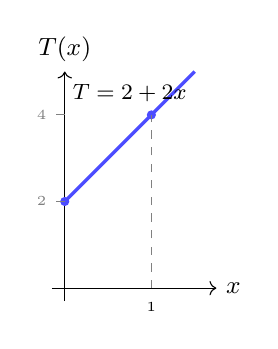
\begin{tikzpicture}[scale=0.55]
    % Optimal map
    \draw[->] (-0.3,0) -- (3.5,0) node[right] {\small $x$};
    \draw[->] (0,-0.3) -- (0,5) node[above] {\small $T(x)$};

    % T(x) = 2 + 2x
    \draw[blue!70, very thick, domain=0:1.5] plot (\x*2, {2 + 2*\x});

    % Reference points
    \fill[blue!70] (0, 2) circle (3pt);
    \fill[blue!70] (2, 4) circle (3pt);

    \node[font=\footnotesize] at (1.5, 4.5) {$T = 2 + 2x$};

    % Dashed guides
    \draw[gray, dashed] (0, 2) -- (-0.2, 2) node[left, font=\tiny] {$2$};
    \draw[gray, dashed] (0, 4) -- (-0.2, 4) node[left, font=\tiny] {$4$};
    \draw[gray, dashed] (2, 0) -- (2, 4);
    \node[below, font=\tiny] at (2, -0.1) {$1$};
\end{tikzpicture}

\vspace{0.3cm}
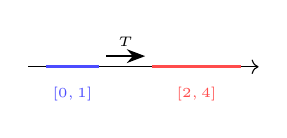
\begin{tikzpicture}[scale=0.45]
    % Source and target on real line
    \draw[->] (-0.5,0) -- (6,0);

    \draw[blue!70, very thick] (0,0) -- (1.5,0);
    \node[below, font=\tiny, blue!70] at (0.75, -0.3) {$[0,1]$};

    \draw[red!70, very thick] (3,0) -- (5.5,0);
    \node[below, font=\tiny, red!70] at (4.25, -0.3) {$[2,4]$};

    \draw[-{Stealth}, thick] (1.7, 0.3) -- (2.8, 0.3);
    \node[above, font=\tiny] at (2.25, 0.3) {$T$};
\end{tikzpicture}
\end{center}
\end{column}
\end{columns}
\end{frame}

%==============================================================================
\begin{frame}{Exercise 3: $c$-Concavity for Quadratic Cost}
\textbf{Problem:} For $c(x,y) = \frac{1}{2}|x-y|^2$, let $\chi(x) = ax$ for $a \in \R$ (in 1D).

\vspace{0.3cm}
\textbf{Questions:}
\begin{enumerate}
    \item[(a)] Compute $u_\chi(x) = \frac{1}{2}x^2 - \chi(x)$.
    \item[(b)] Compute the Legendre transform $(u_\chi)^*(y)$.
    \item[(c)] Verify $\chi^c(y) = \frac{1}{2}y^2 - (u_\chi)^*(y)$ directly from definition.
    \item[(d)] Is $\chi$ a $c$-concave function?
\end{enumerate}

\vspace{0.5cm}
\textit{Hint:} Recall $f^*(y) = \sup_x [xy - f(x)]$ is the Legendre transform.
\end{frame}

%==============================================================================
\begin{frame}{Solution 3}
\textbf{(a)} $u_\chi(x) = \frac{1}{2}x^2 - ax$

\vspace{0.2cm}
\textbf{(b)} $(u_\chi)^*(y) = \sup_x \left[xy - \frac{1}{2}x^2 + ax\right] = \sup_x \left[(y+a)x - \frac{1}{2}x^2\right]$

Maximizing: $x^* = y + a$, so:
\[
(u_\chi)^*(y) = (y+a)^2 - \frac{1}{2}(y+a)^2 = \frac{1}{2}(y+a)^2
\]

\vspace{0.2cm}
\textbf{(c)} Direct computation:
\[
\chi^c(y) = \inf_x \left[\frac{1}{2}(x-y)^2 - ax\right]
\]
Setting derivative to zero: $x^* = y + a$
\[
\chi^c(y) = \frac{1}{2}(y+a-y)^2 - a(y+a) = \frac{a^2}{2} - ay - a^2 = -ay - \frac{a^2}{2}
\]
Verify: $\frac{1}{2}y^2 - (u_\chi)^*(y) = \frac{1}{2}y^2 - \frac{1}{2}(y+a)^2 = -ay - \frac{a^2}{2}$ \checkmark

\vspace{0.2cm}
\textbf{(d)} $\chi = ax$ is $c$-concave iff $\frac{1}{2}x^2 - ax = u_\chi$ is convex. Since $u_\chi'' = 1 > 0$, \textbf{yes}!
\end{frame}

%==============================================================================
\section{Summary}
%==============================================================================

\begin{frame}{Summary}
\textbf{Main Results for $c(x,y) = h(x-y)$, $h$ strictly convex:}

\vspace{0.2cm}
\begin{itemize}
    \item \textbf{Twist condition:} $y \mapsto \nabla_x c(x_0, y)$ injective
    \item \textbf{Theorem 1.17:} If $\mu \ll \Ld$, optimal map exists:
    \[
    T(x) = x - (\nabla h)^{-1}(\nabla\phi(x))
    \]
    \item \textbf{Uniqueness:} Both of optimal plan and map
\end{itemize}

\vspace{0.3cm}
\textbf{Quadratic Case $c(x,y) = \frac{1}{2}|x-y|^2$:}
\begin{itemize}
    \item $c$-concavity $\Leftrightarrow$ convexity (Proposition 1.21)
    \item \textbf{Brenier:} $T = \nabla u$ for convex $u$
    \item Extends to unbounded domains (Theorem 1.22)
    \item Flat torus case (Theorem 1.25)
\end{itemize}

\vspace{0.3cm}
\textbf{Key Tools:} Rademacher's theorem, semi-concavity, duality
\end{frame}

%==============================================================================
\begin{frame}{Looking Ahead}
\textbf{Next topics:}

\vspace{0.3cm}
\begin{itemize}
    \item \textbf{Section 1.4:} Counter-examples to existence
    \begin{itemize}
        \item When $\mu$ is not absolutely continuous
        \item Costs that don't satisfy twist condition
    \end{itemize}

    \vspace{0.3cm}
    \item \textbf{Section 1.6:} $c$-cyclical monotonicity
    \begin{itemize}
        \item Necessary and sufficient conditions for optimality
        \item Proof of strong duality
    \end{itemize}

    \vspace{0.3cm}
    \item \textbf{Section 1.7:} Polar factorization and further results
\end{itemize}

\vspace{0.4cm}
\textbf{Key question for Section 1.4:} What happens when the assumptions of Theorem 1.17 fail?
\end{frame}

\end{document}
